\documentclass[a4paper, twoside, english]{article}

\usepackage{amsmath}
\usepackage{amsfonts}
\usepackage{ihci}
\usepackage{graphicx}
\usepackage{subfig}
\usepackage{listings}
\usepackage{color}
\usepackage{multirow}
\usepackage[table,xcdraw]{xcolor}

% Unicode workaround for lstlistings
\lstset{literate=
	{á}{{\'a}}1 {é}{{\'e}}1 {í}{{\'i}}1 {ó}{{\'o}}1 {ú}{{\'u}}1
	{Á}{{\'A}}1 {É}{{\'E}}1 {Í}{{\'I}}1 {Ó}{{\'O}}1 {Ú}{{\'U}}1
	{à}{{\`a}}1 {è}{{\`e}}1 {ì}{{\`i}}1 {ò}{{\`o}}1 {ù}{{\`u}}1
	{À}{{\`A}}1 {È}{{\'E}}1 {Ì}{{\`I}}1 {Ò}{{\`O}}1 {Ù}{{\`U}}1
	{ä}{{\"a}}1 {ë}{{\"e}}1 {ï}{{\"i}}1 {ö}{{\"o}}1 {ü}{{\"u}}1
	{Ä}{{\"A}}1 {Ë}{{\"E}}1 {Ï}{{\"I}}1 {Ö}{{\"O}}1 {Ü}{{\"U}}1
	{â}{{\^a}}1 {ê}{{\^e}}1 {î}{{\^i}}1 {ô}{{\^o}}1 {û}{{\^u}}1
	{Â}{{\^A}}1 {Ê}{{\^E}}1 {Î}{{\^I}}1 {Ô}{{\^O}}1 {Û}{{\^U}}1
	{œ}{{\oe}}1 {Œ}{{\OE}}1 {æ}{{\ae}}1 {Æ}{{\AE}}1 {ß}{{\ss}}1
	{ű}{{\H{u}}}1 {Ű}{{\H{U}}}1 {ő}{{\H{o}}}1 {Ő}{{\H{O}}}1
	{ç}{{\c c}}1 {Ç}{{\c C}}1 {ø}{{\o}}1 {å}{{\r a}}1 {Å}{{\r A}}1
	{€}{{\euro}}1 {£}{{\pounds}}1 {«}{{\guillemotleft}}1
	{»}{{\guillemotright}}1 {ñ}{{\~n}}1 {Ñ}{{\~N}}1 {¿}{{?`}}1
}

% Define Synatx highlighting for Python
\definecolor{maroon}{cmyk}{0, 0.87, 0.68, 0.32}
\definecolor{halfgray}{gray}{0.55}
\definecolor{ipython_frame}{RGB}{207, 207, 207}
\definecolor{ipython_bg}{RGB}{247, 247, 247}
\definecolor{ipython_red}{RGB}{186, 33, 33}
\definecolor{ipython_green}{RGB}{0, 128, 0}
\definecolor{ipython_cyan}{RGB}{64, 128, 128}
\definecolor{ipython_purple}{RGB}{170, 34, 255}

\lstdefinelanguage{iPython}{
	morekeywords=[1]{access,and,break,class,continue,def,del,elif,else,except,exec,finally,for,from,global,if,import,in,is,lambda,not,or,pass,print,raise,return,try,while},%
	%
	% Built-ins
	morekeywords=[2]{abs,all,any,basestring,bin,bool,bytearray,callable,chr,classmethod,cmp,compile,complex,delattr,dict,dir,divmod,enumerate,eval,execfile,file,filter,float,format,frozenset,getattr,globals,hasattr,hash,help,hex,id,input,int,isinstance,issubclass,iter,len,list,locals,long,map,max,memoryview,min,next,object,oct,open,ord,pow,property,range,raw_input,reduce,reload,repr,reversed,round,set,setattr,slice,sorted,staticmethod,str,sum,super,tuple,type,unichr,unicode,vars,xrange,zip,apply,buffer,coerce,intern},%
	%
	sensitive=true,%
	morecomment=[l]\#,%
	morestring=[b]',%
	morestring=[b]",%
	%
	morestring=[s]{'''}{'''},% used for documentation text (mulitiline strings)
	morestring=[s]{"""}{"""},% added by Philipp Matthias Hahn
	%
	morestring=[s]{r'}{'},% `raw' strings
	morestring=[s]{r"}{"},%
	morestring=[s]{r'''}{'''},%
	morestring=[s]{r"""}{"""},%
	morestring=[s]{u'}{'},% unicode strings
	morestring=[s]{u"}{"},%
	morestring=[s]{u'''}{'''},%
	morestring=[s]{u"""}{"""},%
	morestring=[s]{f'}{'},% format strings
	morestring=[s]{f"}{"},%
	morestring=[s]{f'''}{'''},%
	morestring=[s]{f"""}{"""},%
	%
	identifierstyle=\color{black}\ttfamily,
	commentstyle=\color{ipython_cyan}\ttfamily,
	stringstyle=\color{ipython_red}\ttfamily,
	keepspaces=true,
	showspaces=false,
	showstringspaces=false,
	%
	rulecolor=\color{ipython_frame},
	frame=single,
	frameround={t}{t}{t}{t},
	framexleftmargin=7mm,
	numbers=left,
	numberstyle=\tiny\color{halfgray},
	%
	%
	backgroundcolor=\color{ipython_bg},
	extendedchars=true,
	%basicstyle={\footnotesize\ttfamily},
	basicstyle={\scriptsize\ttfamily},
	keywordstyle=[1]{\color{ipython_green}\ttfamily},
	keywordstyle=[2]{\color{ipython_purple}\ttfamily},
}

\graphicspath{{./../figures/}}

\title{Machine Learning Project\\Task 3 Report}  
\author{Albert Garaev,\\ Ksenia Novikova,\\ Mukhammadsodik Khabibulloev }    
\date{01.02.2022}                              

\begin{document}

\maketitle

\section{Tabular Reinforcement Learning}

Reinforcement learning is one of the methods of machine learning, during which the system under test (agent) learns by interacting with some environment. The agent and the environment constantly interact, the agent chooses actions, and the environment responds to these actions and presents new situations to the agent. The environment also generates rewards, special numerical values that the agent seeks to maximize through his choice of actions. For instance, escaping from a maze: you need to get the agent to find the exit as soon as possible, so the reward is -1 for each time step leading up to the escape. In a game of chess, the reward is +1 for a win, 0 for a draw, and -1 for a loss. In this case, the reward mechanism that tells the agent what is right and what is wrong, using reward and punishment, will be the reward function. The goal of the agent is to maximize its cumulative reward, called return, where the return is defined as some specific function of the reward sequence. In simple case it might be sum of all rewards. \\


The environment is typically stated in the form of a Markov decision process (MDP). MDP is a classic formalization of sequential decision making. In this case actions affect not only immediate rewards, but also subsequent states or situations, and through these future rewards. Thereby, MDPs include deferred gratification and the need to balance between immediate and deferred gratification. We evaluate the value $q(s, a)$ of each action $a$ in each state $s$, or we evaluate the value $v(s)$ of each state under the optimal choice of action. These state-dependent quantities are needed to accurately determine the long-term consequences of choosing individual actions. ~\cite{MPD}\\

The agent chooses the appropriate strategy (a subset of all possible behaviors) in relation to its goals. Thus, a policy is a strategy that an agent uses to achieve goals. The policy defines the actions that the agent performs based on the state of the agent and the environment. We also need to know about discounting. The discount factor determines how much the agent cares about rewards in the distant future compared to rewards in the near future. The value of the discount rate parameter is $\gamma, \ where \ (0 \leq \gamma \leq 1)$, if $\gamma=0$, the agent will only know about actions that bring an immediate reward. ~\cite{MPD2}\\
Many reinforcement learning algorithms for assessing how well an agent perform a given action in a given state (or simply be in a given state), use the evaluation of value functions $v(s)$, that is, state functions (or pairs of actions and states). It is equal to the expected total reward for the agent, starting from state $s$. The value function depends on the policy according to which the agent chooses the actions to perform. The value function of a state $s$ under a policy $\pi$ is the expected return starting in $s$ and following $\pi$ thereafter. It is denoted $v_\pi(s)$ and called state-value function for policy $\pi$. Similarly, we can define the value of taking action $a$ in state $s$ under a policy $\pi$ as the expected return starting from $s$, taking the action $a$, and thereafter following policy $\pi$. It is denoted $q_\pi(s, a)$ and called action-value function for policy $\pi$.\\
Optimal policy (there may be more than one) is better than or equal to all other policies, denote all the optimal policies by $\pi_*$. 
They have the same state-value function, called the optimal state-value function $v_*(s)$ and optimal action-value function $q_*(s, a)$:  ~\cite{MPD2}\\
$v_*(s)= \underset{\pi}{max} \ v_\pi(s)$\\
$q_*(s, a) = \underset{\pi}{max} \ q_\pi(s, a)$
~\\
~\\
Bellman equation for value function (state-value function): ~\cite{MPD}\\
 $v(s) = \mathbb{E}[R_{t+1}+\gamma \ v(S_{t+1})|S_t=s]$\\
It can be seen from the above equation that the value of the state can be decomposed into the immediate reward (R[t+1]) plus the value of the subsequent state (v[S (t+1)]) with a discount factor $\gamma$. This still means the Bellman expectation equation, but now we are finding the value of a particular state subject to some policy $\pi$. This is the difference between the Bellman equation and the Bellman expectation equation, which can be written as a formula:\\
 $v_\pi(s) = \mathbb{E_\pi}[R_{t+1}+\gamma \ v_\pi(S_{t+1})|S_t=s]$\\
We can observe that in this case the value of a particular state is determined by the immediate reward plus the value of subsequent states following a certain policy $\pi$. \\ 
Similarly, we can write state-action value function (Q-Function):\\
$q_*(s, a) = \mathbb{E}[R_{t+1}+\gamma\underset{a'}{max} \ q_*(S_{t+1}, a')|S_t=s,A_t=a]$\\
From the above equation, we can see that the state-action value  can be decomposed into the immediate reward we get on performing a certain action in state(s) and moving to another state(s') plus the discounted value of the maximum state-action value of the state(s') with respect to the some action(a) our agent will take from that state on-wards.

\subsection{SARSA}
SARSA (State-action-reward-state-action) is the most basic algorithm for learning a Markov decision process policy, used in the reinforcement learning. In SARSA, we use the same policy (e.g. epsilon-greedy) that generated the previous action a to generate the next action, a + 1, which we run through our Q function for updates.the agent forms a utility function Q:\\
$Q[S,A] = Q[S,A] + \alpha(R+\gamma \ Q[S', A'] - Q[S,A])$, where hyperparameters $\alpha$ is the step-size and $\gamma$ the discount factor.\\

 The key difference between SARSA and Q-learning, discussed below, is that it is an on-policy algorithm. This means that SARSA evaluates Q values based on the actions taken by the current policy. 
 %We implement SARSA algorithm:
 %SARSA



%!!!!!!!!!!!!!!!
We implement SARSA algorithm. The full code can be seen in Appendix 1. \ref{App1} Now we can visualize the resulting approximation to the optimal policy by drawing two possible paths that could be taken under that policy. The Figure \ref{fig:path} shows this paths.\\
\begin{figure}[h!]
	\centerline
	{
		\subfloat[]{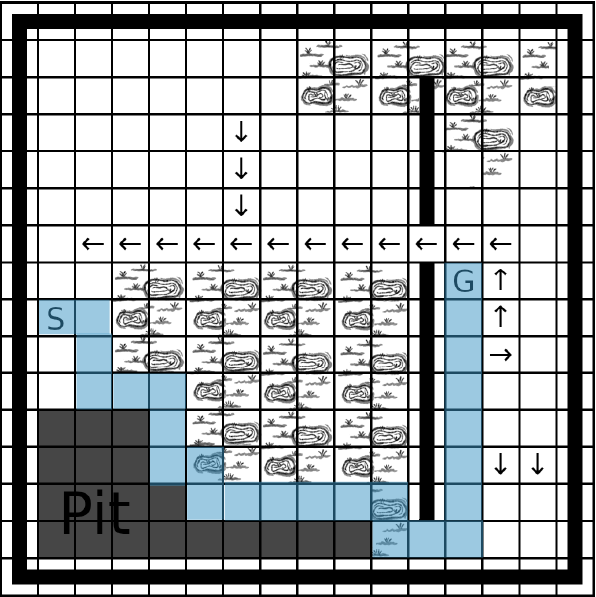
\includegraphics[width=0.40\textwidth]{path1.png}}
		\quad
		\subfloat[]{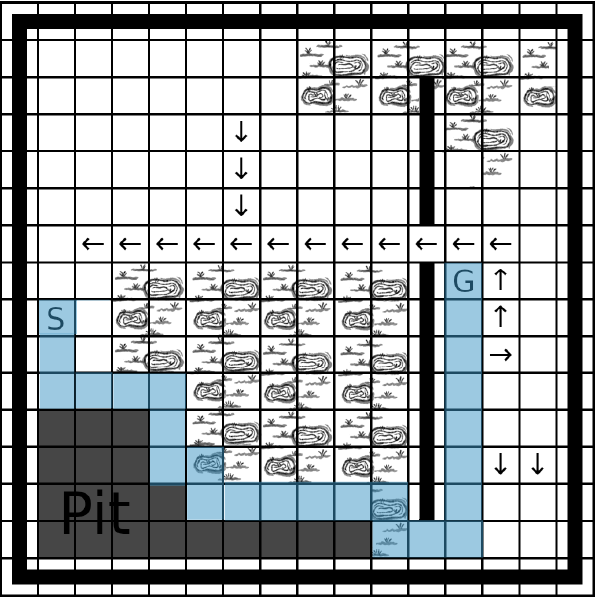
\includegraphics[width=0.40\textwidth]{path2.png}}
	}
	\caption[null]{SARSA. Two possible paths}
	\label{fig:path}
\end{figure}

\newpage

%!!!!!!!!!!!!!!!!!!!!!
We implement alrorithm for our task using different values of $\varepsilon$. The Figure \ref{fig:SARSA1_eps} shows training progress, all episodes on the x-axis and the total return accumulated in that episode on the y-axis.\\


\begin{figure}[h!]
	\centerline
	{
		\subfloat[]{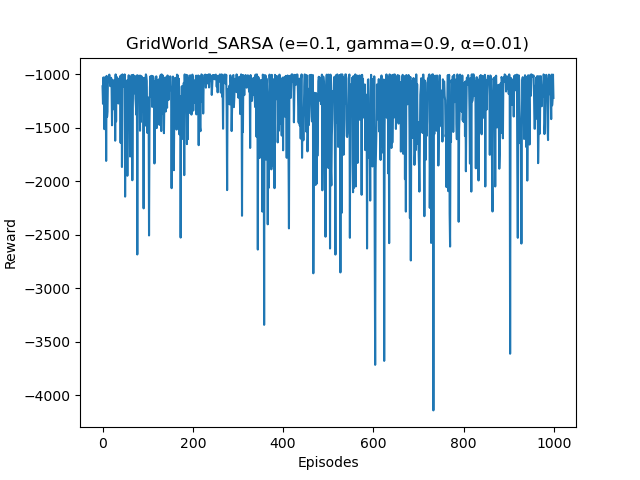
\includegraphics[width=0.40\textwidth]{SARSA_R_1_1.png}}
		\quad
		\subfloat[]{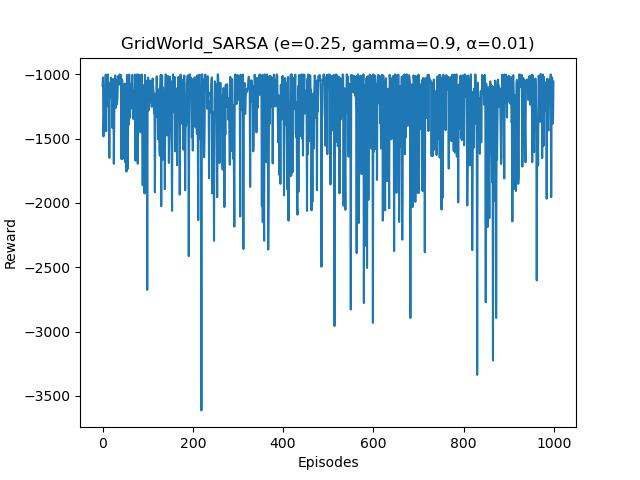
\includegraphics[width=0.40\textwidth]{SARSA_R_1_2.png}}
		\quad
		\subfloat[]{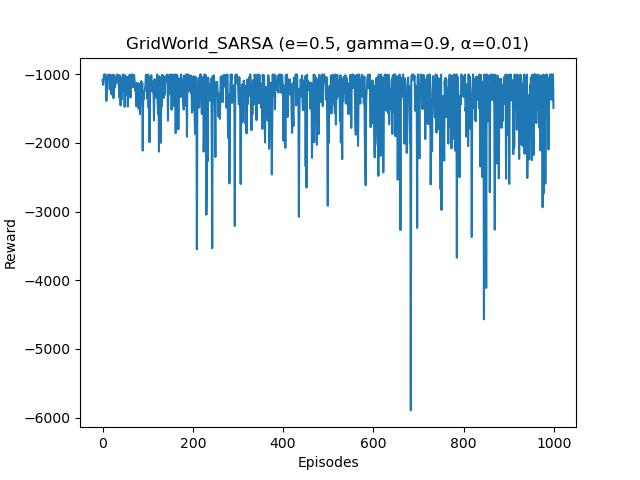
\includegraphics[width=0.40\textwidth]{SARSA_R_1_3.png}}
	}
	\caption[null]{SARSA. Training progress with a) $\varepsilon= 0.1$, b) $\varepsilon= 0.25$, c) $\varepsilon= 0.5$}
	\label{fig:SARSA1_eps}
\end{figure}

Also we try setting $\varepsilon=0$, i.e., the agent deterministically chooses the action with the maximal Q value. 

%!!!!!!!!!!!!Summarize your findings and try to explain the observed behavior.
When $\varepsilon=0$, the agent gets stuck and does not move further. For values of $\varepsilon$ closer to zero, the agent also gets stuck in the same cells. It can be assumed that the reason for this is the fact that when choosing $\varepsilon$ close to or equal to 0, the agent chooses actions with maximum Q, so at certain points in the Gridworld it starts moving within the same cells (our experiments show that getting stuck occurs in cells (14,14), (14,13),(13,14),(13,13),(12,14)), without the ability to get out, since it is for these cells that the value of Q is maximum.\\
In our case, with 1000 episodes, the algorithm does not converge. We ran the algorithm for 10000 episodes, in this case the agent reached the goal only 1 time. The Figure \ref{fig:SARSA_1_10000} shows training progress with 10000 episodes.\\
\begin{figure}[h!]
	\centerline{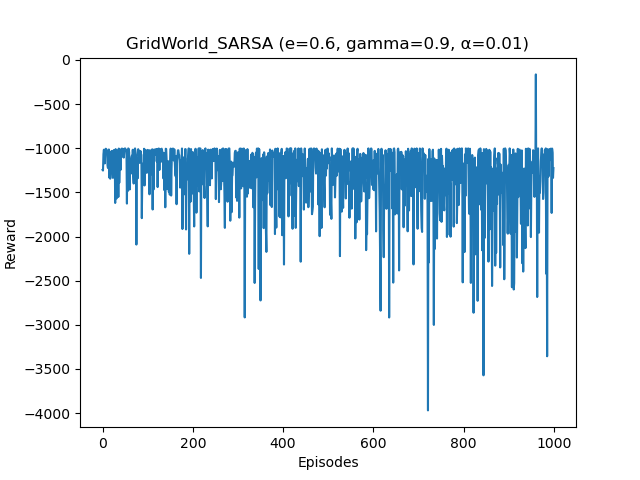
\includegraphics[width=0.45\textwidth]{SARSA_R1_10000.png}}
	\caption[null]{SARSA. Training progress for 10000 episodes $\varepsilon=0.6$}
	\label{fig:SARSA_1_10000}
\end{figure}
~\\
The rules for our reward function in this case: receive a reward of -1 in each time step, except for falling into the pits, which incurs a penalty of -1000. This reward function is not well suited for our promlem.

\newpage

%Q-lern!!!!!!!!!!!!!!!!1

\subsection{Q-Learning}
Q-learning is a method used in artificial intelligence with an agent-based approach. Refers to reinforcement learning experiments. Based on the reward received from the environment, the agent forms a utility function Q:\\
$Q[S,A] = Q[S,A] + \alpha(R+\gamma \ \underset{a}{max}Q[S', a] - Q[S,A])$, where hyperparameters $\alpha$ is the step-size and $\gamma$ the discount factor.\\

This function subsequently gives to agent the opportunity not to randomly choose a behavior strategy, but to take into account the experience of previous interaction with the environment. One of the advantages of Q-learning is that it is able to compare the expected utility of available activities without having to model the environment. It is used for situations that can be represented as a Markov decision process. Note that the next action is chosen to maximize the Q-value of the next states instead of following the current policy. As a result, Q-learning is categorized as off-Policy.\\
We implement Q-Learning algorithm. The full code can be seen in Appendix 2. \ref{App2}\\
%Q-Learn
After that we implement alrorithm for our task using different values of $\varepsilon$. The Figure \ref{fig:Q_Learn1_eps} shows training progress, all episodes on the x-axis and the total return accumulated in that episode on the y-axis.\\

\begin{figure}[h!]
	\centerline
	{
		\subfloat[]{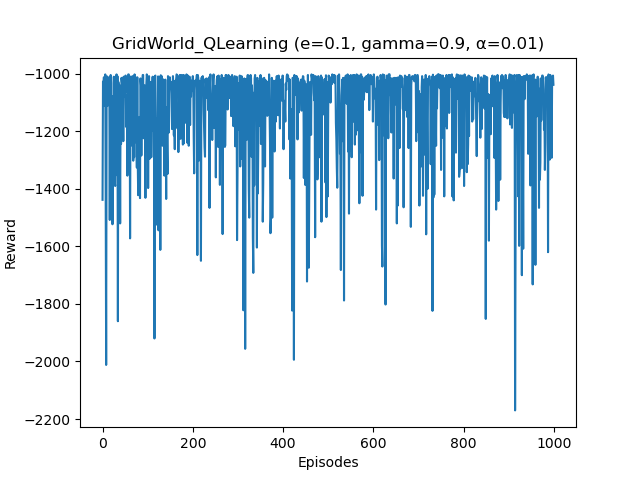
\includegraphics[width=0.40\textwidth]{Qlearn_R_1_1.png}}
		\quad
		\subfloat[]{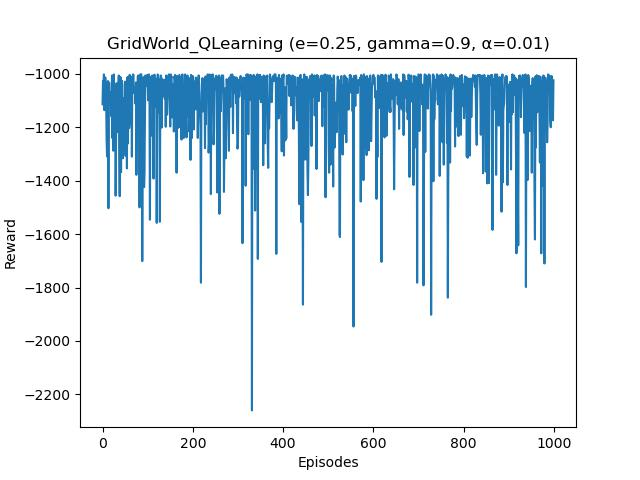
\includegraphics[width=0.40\textwidth]{Qlearn_R_1_2.png}}
		\quad
		\subfloat[]{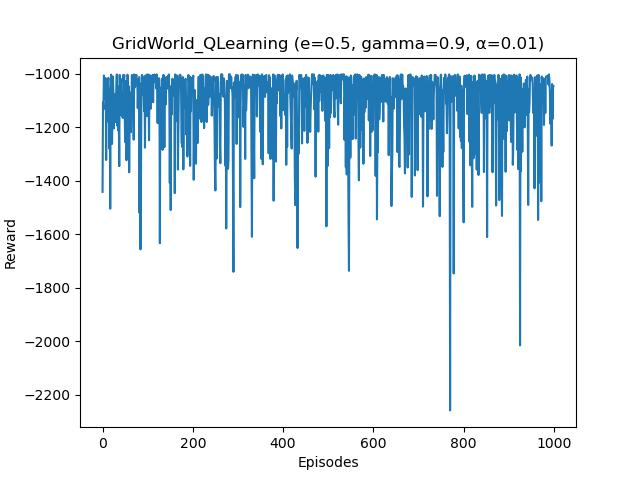
\includegraphics[width=0.40\textwidth]{Qlearn_R_1_3.png}}
	}
	\caption[null]{Q-Learning. Training progress with a) $\varepsilon= 0.1$, b) $\varepsilon= 0.25$, c) $\varepsilon= 0.5$}
	\label{fig:Q_Learn1_eps}
\end{figure}

%!!!!!!!!!!!!Summarize your findings and try to explain the observed behavior.
Also we try setting $\varepsilon=0$, i.e., the agent deterministically chooses the action with the maximal Q value. In our case, with 1000 episodes, the algorithm does not converge. We ran the algorithm for 10000 episodes, in this case the agent also didn't reach the goal. The Figure \ref{fig:Q_Learn1_10000} shows training progress with 10000 episodes.\\
\begin{figure}[h!]
	\centerline{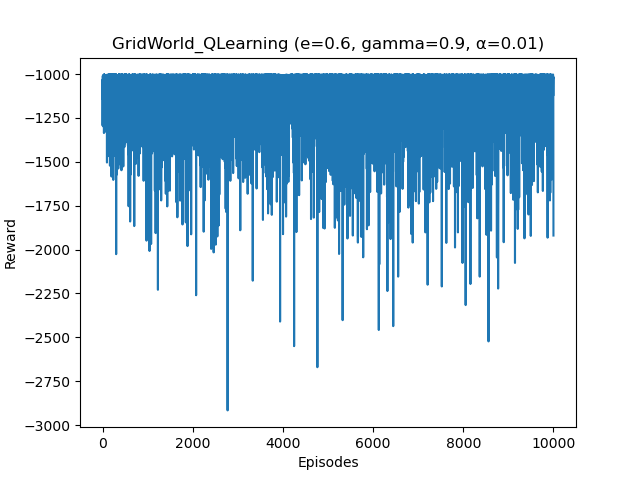
\includegraphics[width=0.40\textwidth]{Qlearn_R1_10000.png}}
	\caption[null]{Q-Learning. Training progress for 10000 episodes $\varepsilon=0.6$}
	\label{fig:Q_Learn1_10000}
\end{figure}

The rules for our reward function is the same as SARSA: receive a reward of -1 in each time step, except for falling into the pits, which incurs a penalty of -1000. This reward function is not well suited for our promlem.\\
%This reward function is not suitable for our case.

\newpage

\subsection{SARSA and Q-Learning comparasion}
As we know, the goal of our Gridworld problem is for the agent to reach the goal state, and we cannot explicitly declare the goal to the agent within the reinforcement learning. However, we need to encode this goal into a reward function, which the agent then tries to maximize over time. We specified reward function in our case. Howewer, is not the only possible way. The first one is our innitially defaulted function and another is two alternativies.\\
~\\
1. The agent receives a reward of -1 in each time step, except for falling into the pits, which incurs a penalty of -1000.\\
2. The agent receives no reward (i.e., 0) on each time step, except when reaching the goal, which gives a reward of 1. Falling into the pits is still punished with a reward of -1000.\\
3. Pits remain the same as in the previous two choices, however the agent receives the negative Manhattan distance from its current position to the goal as a reward. More speciffically, if the agent moves to position $(x_a, y_a)$ and the goal is at $(x_g, y_g)$, the reward will be $R=-|x_g-x_a|-|y_g-y_a|$\\
~\\

%Think about it. 1.Time 2. Only goal 3. Distance

We can see that the first reward function imposes restrictions on the agent in terms of execution time (or number of steps), the only goal of the second function is for the agent to reach the goal without additional restrictions. In the third case, it is important for the agent to minimize the Manhattan distance to the target. Note that for all reward functions, there is still a restriction in the form of hitting a "pit". We can make assumptions that in cases where only the achievement of the goal is important, without additional restrictions, the second reward function shows the best result.\\

After that we implement new reward functions 2 and 3 to check our hypotheses. The Table shows the comparisions of results for all reward functions and also for different $\varepsilon$.
We can see results in Table \ref{table:1}\\
% Please add the following required packages to your document preamble:
% \usepackage{multirow}
\begin{table}[h!]
	\begin{tabular}{ccccccc}
		\multicolumn{7}{c}{SARSA}                                                                                                                                                                                                                                      \\
		\multicolumn{1}{l} {\textbf{Reward function}} & {\textbf{Episod number}} & \multicolumn{1}{l}{\textbf{$\varepsilon$}} & \multicolumn{1}{l}{\textbf{$\gamma$}} & \multicolumn{1}{l}{\textbf{$\alpha$}} & \multicolumn{1}{l}{\textbf{time (sec.)}} & \multicolumn{1}{l}{\textbf{finish}} \\
		\multirow{4}{*}{1}                  & \multirow{4}{*}{1000}  & 0.1                                  & 0.9                                & 0.01                               & 123.49                                   & 0                                   \\
		&                        & 0.25                                 & 0.9                                & 0.01                               & 122.72                                   & 0                                   \\
		&                        & 0.5                                  & 0.9                                & 0.01                               & 135.94                                   & 0                                   \\
		&                        & 0                                    & 0.9                                & 0.01                               & 135.94                                   & 0                                   \\
		\multirow{4}{*}{2}                  & \multirow{4}{*}{1000}  & 0.1                                  & 0.9                                & 0.01                               & -                                        & -                                   \\
		&                        & 0.25                                 & 0.9                                & 0.01                               & 1871.1                                   & 426                                 \\
		&                        & 0.5                                  & 0.9                                & 0.01                               & 954.26                                   & 0                                   \\
		&                        & 0                                    & 0.9                                & 0.01                               & -                                        & -                                   \\
		\multirow{4}{*}{3}                  & \multirow{4}{*}{1000}  & 0.1                                  & 0.9                                & 0.01                               & 68                                       & 0                                   \\
		&                        & 0.25                                 & 0.9                                & 0.01                               & 69.12                                    & 0                                   \\
		&                        & 0.5                                  & 0.9                                & 0.01                               & 89.6                                     & 2                                   \\
		&                        & 0                                    & 0.9                                & 0.01                               & -                                        & -                                  
	\end{tabular}
	\caption{Comparasion of reward functions for SARSA algorithm}
	\label{table:1}
\end{table}

\newpage

We do the same comparasion for Q-Learning. The results can be seen in Table \ref{table:2}\\
\begin{table}[h!]
	\begin{tabular}{ccccccc}
		\multicolumn{7}{c}{Q-Learning}                                                                                                                                                                                                                                 \\
		\multicolumn{1}{l} {\textbf{Reward function}} & {\textbf{Episod number}} & \multicolumn{1}{l}{\textbf{$\varepsilon$}} & \multicolumn{1}{l}{\textbf{$\gamma$}} & \multicolumn{1}{l}{\textbf{$\alpha$}} & \multicolumn{1}{l}{\textbf{time (sec.)}} & \multicolumn{1}{l}{\textbf{finish}} \\
		\multirow{4}{*}{1}                  & \multirow{4}{*}{1000}  & 0.1                                  & 0.9                                & 0.01                               & 36.94                                    & 0                                   \\
		&                        & 0.25                                 & 0.9                                & 0.01                               & 33.33                                    & 0                                   \\
		&                        & 0.5                                  & 0.9                                & 0.01                               & 31.77                                    & 0                                   \\
		&                        & 0                                    & 0.9                                & 0.01                               & -                                        & -                                   \\
		\multirow{4}{*}{2}                  & \multirow{4}{*}{1000}  & 0.1                                  & 0.9                                & 0.01                               & -                                        & -                                   \\
		&                        & 0.25                                 & 0.9                                & 0.01                               & -                                        & -                                   \\
		&                        & 0.5                                  & 0.9                                & 0.01                               & 915.9                                    & 0                                   \\
		&                        & 0                                    & 0.9                                & 0.01                               & -                                        & -                                   \\
		\multirow{4}{*}{3}                  & \multirow{4}{*}{1000}  & 0.1                                  & 0.9                                & 0.01                               & 40.2                                     & 0                                   \\
		&                        & 0.25                                 & 0.9                                & 0.01                               & 40.3                                     & 0                                   \\
		&                        & 0.5                                  & 0.9                                & 0.01                               & 38.13                                    & 0                                   \\
		&                        & 0                                    & 0.9                                & 0.01                               & -                                        & -                                  
	\end{tabular}
	\caption{Comparasion of reward functions for Q-Learnig algorithm}
	\label{table:2}
\end{table}



As we can see results are also unsatisfactory. So we try to make more episodes for reward functions.  Table \ref{table:3} shows the results with 10000 episodes for SARSA and Q-Learning algorithms.\\
\begin{table}[h!]
	\begin{tabular}{cccccll}
		\multicolumn{1}{l}{\textbf{Reward function}} & \textbf{Episod number} & \multicolumn{1}{l}{\textbf{$\varepsilon$}} & \multicolumn{1}{l}{\textbf{$\gamma$}} & \multicolumn{1}{l}{\textbf{$\alpha$}} & \textbf{time (sec.)} & \textbf{finish} \\
		\multicolumn{7}{c}{\cellcolor[HTML]{CBCEFB}SARSA}                                                                                                                                                                               \\
		1                                            & 10000                  & 0.6                                  & 0.9                                & 0.01                               & 117.4                & 1               \\
		2                                            & 10000                  & 0.6                                  & 0.9                                & 0.01                               & 442.4                & 12              \\
		3                                            & 10000                  & 0.6                                  & 0.9                                & 0.01                               & 88.17                & 0               \\
		\multicolumn{7}{c}{\cellcolor[HTML]{CBCEFB}Q-Learning}                                                                                                                                                                          \\
		1                                            & 10000                  & 0.6                                  & 0.9                                & 0.01                               & 320.74               & 0               \\
		2                                            & 10000                  & 0.6                                  & 0.9                                & 0.01                               & 162.6                & 3338            \\
		3                                            & 10000                  & 0.6                                  & 0.9                                & 0.01                               & 362.15               & 1              
	\end{tabular}
	\caption{Comparasion of reward functions for SARSA algorithm}
	\label{table:3}
\end{table}
~\\
Now we can see that better results show the second reward function. The time of working is 162.6 seconds and 3338 times agent reached the goal with 10000 episodes.
As stated above, this kind of reward function shows better results, because the only goal of this function is for the agent to reach the goal, and we do not care about the elapsed time (number of steps) nor the Manhattan distance to the goal. So in cases, in cases where only achieving the goal is important, without additional restrictions, this reward function shows the best result.


%!!!!!!!!!!!!Bellman optimality

We can write Bellman equation for state-action value function (Q-Function):\\
$q_*(s, a) = \mathbb{E}[R_{t+1}+\gamma\underset{a'}{max} \ q_*(S_{t+1}, a')|S_t=s,A_t=a]$\\
Bellman equation  tells that the value of an action a in some state s is the immediate reward you get for taking that action, to which you add the maximum expected reward you can get in the next state. We can compute the optimal action-value function $q_*$ for our tasks using this equation.

\newpage

\section{Deep Reinforcement Learning}
%task 2a
We implement a discretization of the state space of the cart-pole problem. \\
Hyperparameters: number of episodes	50000, $\varepsilon$ 0.2, $\gamma$ (discount factor) 0.9, $\alpha$ (learning rate) 0.25\\
Figure \ref{fig:deep_learn1} shows results when running it along with SARSA and Q-learning. \\

\begin{figure}[h!]
	\centerline
	{
		\subfloat[]{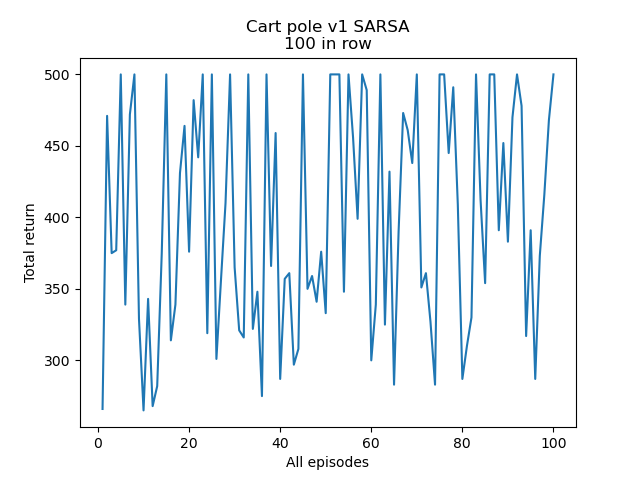
\includegraphics[width=0.40\textwidth]{Cart_Pole_SARSA_50000_in_row.png}}
		\quad
		\subfloat[]{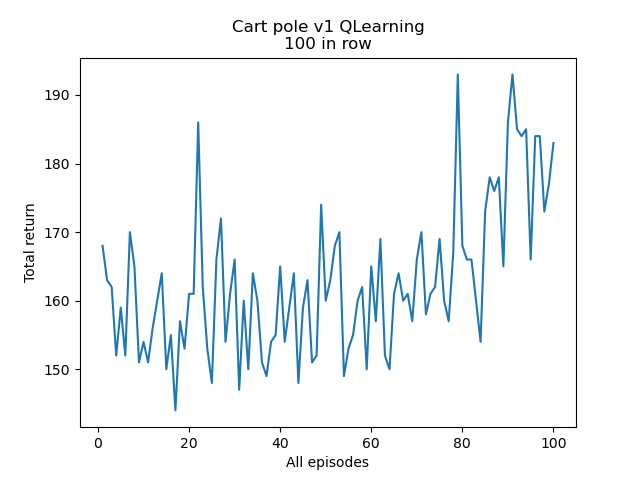
\includegraphics[width=0.40\textwidth]{Cart_Pole_QL_0_50000_in_row.png}}
	}
	\caption[null]{Visualization for 100 episodes in a row for a) SARSA, b) Q-Learning}
	\label{fig:deep_learn1}
\end{figure}
 As can be seen from the figures above, as well as from the output of the program, for SARSA, the average reward value is 368, for Q-Learning 163. Thus, we can conclude that the problem was solved only by the SARSA method, since the reward value for 100 episodes in a row over 195. Also we can compare the elapsed time for SARSA 697.95 seconds, for Q-Learning 376.917 seconds. Although the Q-Learning algorithm shows betters results in time, we cannot called this method solving our problem.
 
We implement deep Q-Learning by replacing the original update rule with the simple neural network and the lookup table Q with calls to the prediction function of the neural network. We use simple, fully-connected neural network with two hidden layers to solve the cart-pole problem. \\


\begin{lstlisting}[language=iPython]
  self.network = nn.Sequential(
  	nn.Linear(self.inputs, 16, bias=True),
  	nn.ReLU(),
  	nn.Linear(16, 16, bias=True),
  	nn.ReLU(),
  	nn.Linear(16, 16, bias=True),
  	nn.ReLU(),
  	nn.Linear(16, self.outputs, bias=True))
  	
  if self.device == 'cuda':
  	self.network.cuda()
  	
  self.optimizer = torch.optim.Adam(self.parameters(),
  	lr=self.learning_rate)
\end{lstlisting}

\newpage

Table \ref{table:4} shows the results for Deep Q-Learning.\\

\begin{table}[h!]
	\begin{tabular}{lll}
		\multicolumn{1}{c}{\textbf{$\varepsilon$}} & \textbf{time (sec.)} & \textbf{number of episodes to finish} \\
		0                                & 57.386703            & 820                                   \\
		0.1                              & 52.873379            & 745                                   \\
		0.2                              & 58.156106            & 736                                   \\
		0.25                             & 57.995978            & 655                                   \\
		0.5                              & Not solved           & Not solved                           
	\end{tabular}
	\caption{Comparasion of time and number of episodes for deep Q-learning}
	\label{table:4}
\end{table}

However, training has become unstable, due to the fact that now one update for a particular action-value pair can affect the approximate values of q for many other state-value pairs, since all the weights of the networks can depend on update. 
We use Experience Replay to solve this problem. During Experience replay, the algorithm remembers all the state transitions that took place during the operation and trains on them all. In this case we can still perform an update in every time step, but we could also decide to update the network's weights only every few time steps. For our task we choose to update the network's weights every 4 time steps. Table \ref{table:5} shows the results for Deep Q-Learning using Experience replay.\\

\begin{table}[h!]
	\begin{tabular}{lll}
		\multicolumn{1}{c}{\textbf{$\varepsilon$}} & \textbf{time (sec.)} & \textbf{number of episodes to finish} \\
		0                                & 22.952246            & 1253                                  \\
		0.1                              & 20.169345            & 876                                   \\
		0.2                              & 27.047348            & 862                                   \\
		0.25                             & 21.9768128           & 853                                   \\
		0.5                              & Not solved           & Not solved                           
	\end{tabular}
	\caption{Comparasion of time and number of episodes for deep Q-learning using Experience replay}
	\label{table:5}
\end{table}

The Figure \ref{fig:deepQ} shows training progress for Deep Q-Learning, all episodes on the x-axis and the total return accumulated in that episode on the y-axis.\\

\begin{figure}[h!]
	\centerline
	{
		\subfloat[]{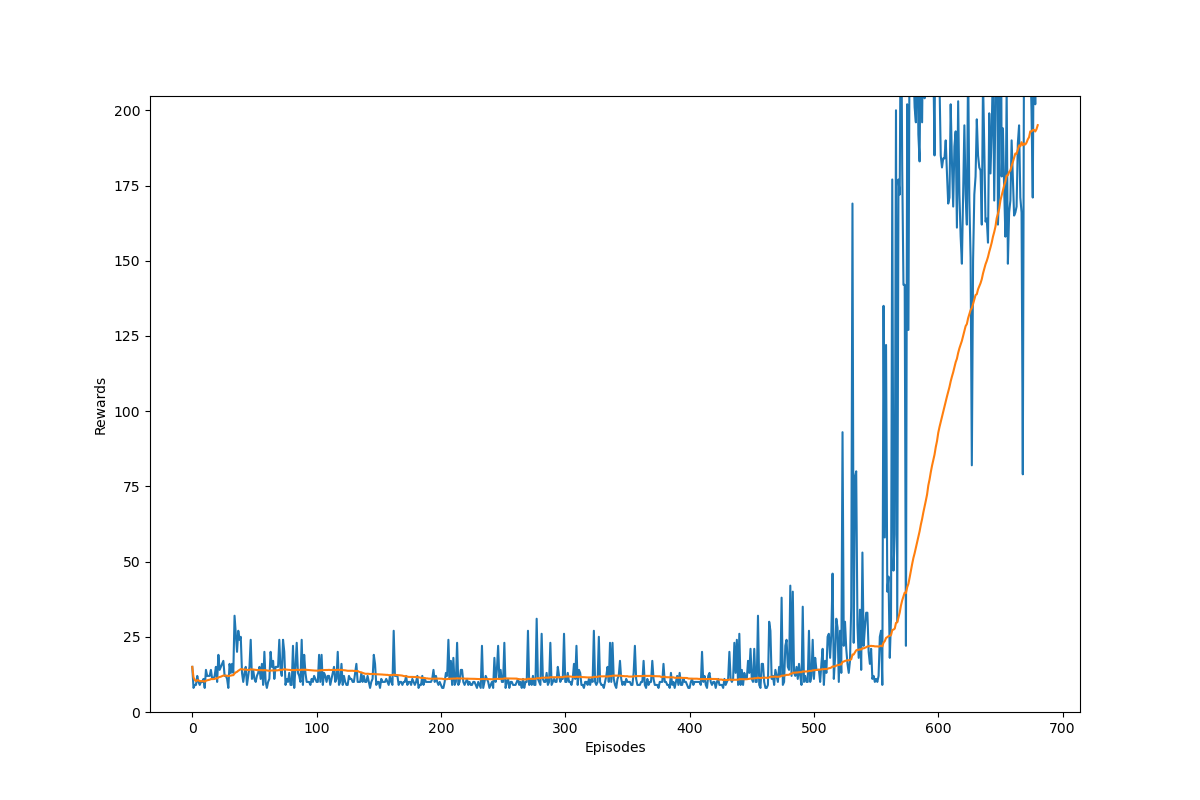
\includegraphics[width=0.40\textwidth]{deepQlearn_0.1.png}}
		\quad
		\subfloat[]{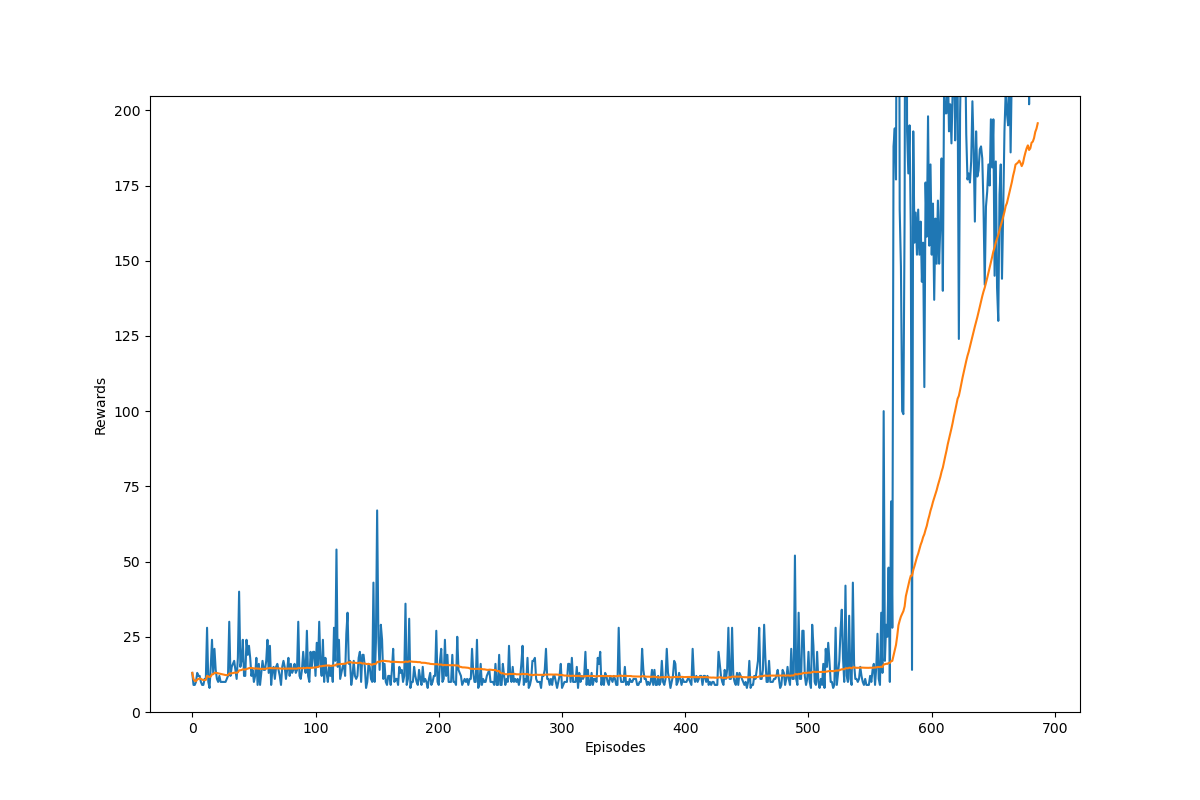
\includegraphics[width=0.40\textwidth]{deepQlearn_0.2.png}}
		\quad
		\subfloat[]{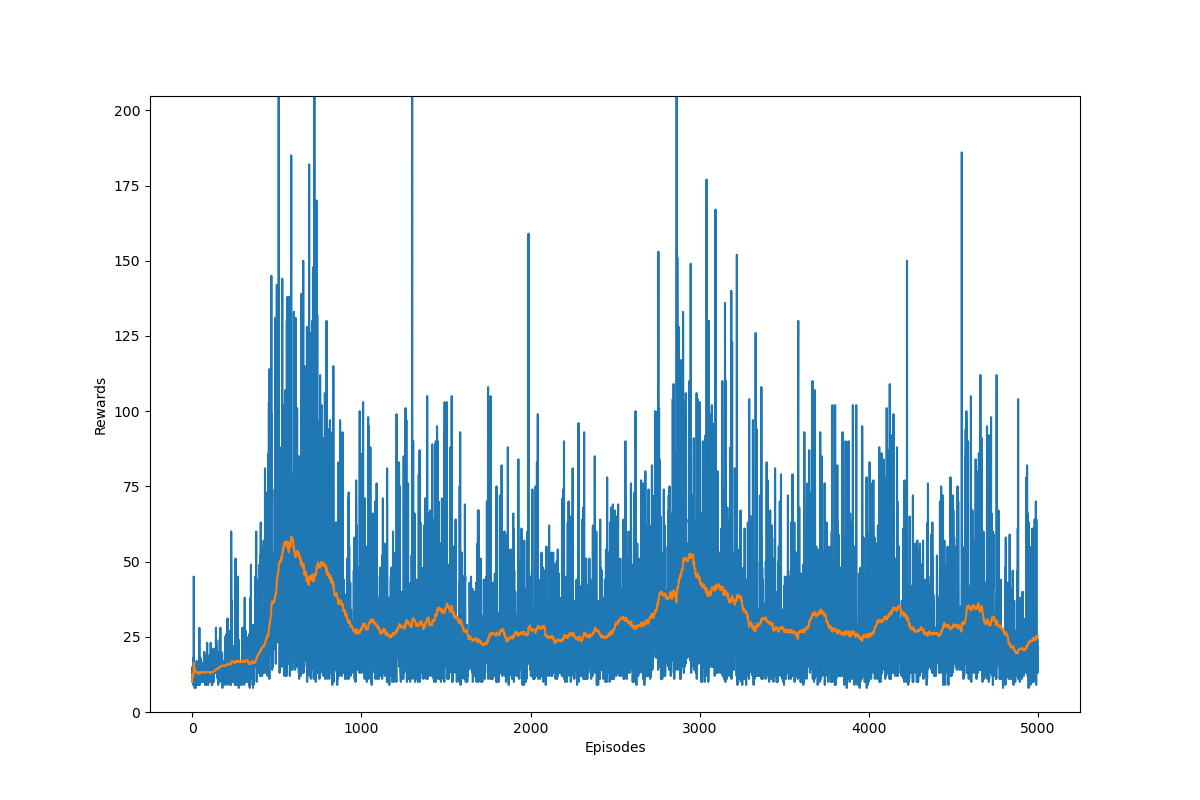
\includegraphics[width=0.40\textwidth]{deepQlearn_0.5.png}}
	}
	\caption[null]{Deep Q-Learnig. Training progress with a) $\varepsilon= 0.1$, b) $\varepsilon= 0.2$, c) $\varepsilon= 0.5$}
	\label{fig:deepQ}
\end{figure}
~\\
As we can see, for our task, deep Q-Learning shows good results: the running time of the algorithm, as well as the number of episodes for which the agent reaches the goal, has decreased. However, we can notice that for epsilon=0.5 the task cannot be solved, the reason for this may be the fact that for the cart-pole task at epsilon 0.5 the algorithm does not cycle, and the reason may be a simple lack of computing power of the laptop on which the experiments were carried out.\\

\bibliographystyle{plain}
\bibliography{bibliography.bib}

\newpage
\section*{Appendix 1} \label{App1}
Implementation for SARSA algorithm\\
\begin{lstlisting}[language=iPython]
	def SarsaTable(num_of_episodes, e_greedy, discount_factor, learning_rate,
	 print_matrix=False):
		world = World.load_from_file('world.json')
		world.reset()
		
		print(f'Starting at pos. ({world.current_state.y},
		 {world.current_state.x}).')
		
		actions = ['right', 'left', 'up', 'down']
		ep_returns = []
		mtx_of_Q_val = np.zeros((4, 16, 16))
		finish = 0
		last_termination = 0
		
		future_action=[]
		for i in range(num_of_episodes):
			print(f'Step {i + 1}/{num_of_episodes}...')
			done = False
			ep_return = 0
			first_case=True
			while (done != True):
				current_state = [world.current_state.y, world.current_state.x]
				if first_case:
					if (random.random() < e_greedy):
						action = random.choice(actions)
					# not random case
					else:
						directions_of_Q_values = mtx_of_Q_val[:, current_state[0],
						 current_state[1]]
						action = actions[
						np.argmax(directions_of_Q_values)]
						first_case=False
				else:
					action = future_action
	
				# the action already chosen
				new_state_all_info, reward, done = world.step(action)
				new_state = [world.current_state.y, world.current_state.x]
				
				if (random.random() < e_greedy):
				future_action = random.choice(actions)
				# not random case
				else:
				directions_of_Q_values = mtx_of_Q_val[:, new_state[0], 
				new_state[1]]
				future_action = actions[
				np.argmax(directions_of_Q_values)]
	
	
	
				if(current_state!=new_state):
					ep_return+=reward
					print(f"\nGoing " + str(action) + " also future action is "
					 + str(future_action))
					print(f'Received a reward of {reward}!')
					print(f'New position is ({new_state_all_info.y}, {new_state_all_info.x})
					 on a {type(new_state_all_info).__name__}.')
					idx_of_dirctn = np.array(np.where(np.array(actions) == action))
					idx_of_dirctn = idx_of_dirctn[0][0]
					
					# Q[S';A']
					# getting a index of new action in new direction
					index_of_new_direction = np.array(np.where(np.array(actions) ==
					 future_action))
					index_of_new_direction = index_of_new_direction[0][0]
					
					mtx_of_Q_val[idx_of_dirctn, current_state[0], current_state[1]] =
					 mtx_of_Q_val[
					idx_of_dirctn,
					current_state[0],
					current_state[1]
					] + learning_rate * (
					reward + discount_factor *
					mtx_of_Q_val[
					index_of_new_direction,
					new_state[0],
					new_state[1]] -
					mtx_of_Q_val[
					idx_of_dirctn,
					current_state[
					0],
					current_state[
					1]])
					
					if done:
						print(f'Episode terminated after {i + 1 - 
							last_termination} steps. Total Return was {ep_return}.')
						if type(new_state_all_info).__name__ == "GoalCell":
						finish += 1
						last_termination = i + 1
						print(f'Resetting the world...')
						world.reset()
			ep_returns.append(ep_return)
	if print_matrix:
		for i in range(len(mtx_of_Q_val)):
			print(actions[i])
				for j in range(len(mtx_of_Q_val[0])):
					for k in range(len(mtx_of_Q_val[0,0])):
						print(str(round(int(mtx_of_Q_val[i,j, k]*10))/10)+" ",end="")
					print()
	
	return ep_returns, finish
\end{lstlisting}	

\newpage
\section*{Appendix 2} \label{App2}
Implementation for Q-Learning algorithm\\
\begin{lstlisting}[language=iPython]
	def QLearningTable(num_of_episodes, e_greedy, discount_factor, learning_rate,
	 print_matrix=False):
	world = World.load_from_file('world.json')
	world.reset()
	
	print(f'Starting at pos. ({world.current_state.y}, {world.current_state.x}).')
	
	actions = ['right', 'left', 'up', 'down']
	ep_returns = []
	mtx_of_Q_val = np.zeros((4, 16, 16))
	finish = 0
	last_termination = 0
	
	for i in range(num_of_episodes):
		print(f'Step {i + 1}/{num_of_episodes}...')
		
		done = False
		ep_return = 0
		while (done != True):
			current_state = [world.current_state.y, world.current_state.x]
			
			if (random.random() < e_greedy):
			action = random.choice(actions)
			# not random case
			else:
			directions_of_Q_values = mtx_of_Q_val[:, current_state[0], 
			current_state[1]]
			action = actions[
			np.argmax(directions_of_Q_values)]
			
			
			# the action already chosen
			new_state_all_info, reward, done = world.step(action)
			new_state = [world.current_state.y, world.current_state.x]
			
			#Bellman
			mtx_of_Q_val = reward + discount_factor * max(qtable[next_state])
			
			if(current_state != new_state):
				ep_return += reward
				
				print(f"\nGoing " + str(action))
				print(f'Received a reward of {reward}!')
				print(f'New position is ({new_state_all_info.y}, {new_state_all_info.x})
				 on a {type(new_state_all_info).__name__}.')
				
				
				idx_of_dirctn = np.array(np.where(np.array(actions) == action))
				idx_of_dirctn = idx_of_dirctn[0][0]
				
				new_state_values = mtx_of_Q_val[:, new_state[0], new_state[1]]
				max_val_in_new_state = new_state_values[np.argmax(new_state_values)]
				
				mtx_of_Q_val[idx_of_dirctn, current_state[0], current_state[1]] = 
				mtx_of_Q_val[
				idx_of_dirctn,
				current_state[0],
				current_state[1]
				] + learning_rate * (
				reward + discount_factor * max_val_in_new_state -
				mtx_of_Q_val[
				idx_of_dirctn,
				current_state[
				0],
				current_state[
				1]])
				
				
				if done:
					print(f'Episode terminated after {i + 1 -
						 last_termination} steps. Total Return was {ep_return}.')
					if type(new_state_all_info).__name__ == "GoalCell":
					finish += 1
					print(f'Resetting the world...')
					world.reset()
			ep_returns.append(ep_return)
		if print_matrix:
			for i in range(len(mtx_of_Q_val)):
				print(actions[i])
					for j in range(len(mtx_of_Q_val[0])):
						for k in range(len(mtx_of_Q_val[0, 0])):
							print(str(round(int(mtx_of_Q_val[i, j, k] * 10)) / 10) +
							 " ", end="")
						print()
	return ep_returns, finish
\end{lstlisting}	

\end{document}